\documentclass{beamer}
\usepackage[english]{babel}
\usepackage{color}
\usepackage{amsfonts}
\usepackage{amssymb}
\usepackage{epsfig}
\usepackage{amsmath}
\usepackage{txfonts}
\usepackage{relsize}
\usepackage{physics}
\bibliographystyle{apalike}
\usepackage{tikz}
\usepackage{ifthen}
\usepackage{caption,subcaption}
\usepackage{svg}
\usetikzlibrary{decorations.pathreplacing,arrows.meta}
\usepackage[style=verbose,backend=bibtex]{biblatex}

%\usepackage{bbold}
\usepackage{dsfont}
\usepackage{bbm}

\usepackage[latin1]{inputenc}

\newcommand{\id}{\mathbbm{1}}
\newcommand{\HH}{\mathcal{H}}
\newcommand{\CC}{\mathbb{C}}
\newcommand{\BB}{\mathcal{B}}
\newcommand{\UU}{\mathcal{U}}
\newcommand{\ZZ}{\mathbb{Z}}
\renewcommand{\AA}{\mathcal{A}}
\newcommand{\Ad}[1]{\textrm{Ad}\left(#1\right)}

\newcommand{\mean}[1]{\langle #1 \rangle}
\newcommand{\cumul}[1]{\langle\!\langle #1 \rangle\!\rangle}

\renewcommand{\d}{\textrm{d}}

\DeclareRobustCommand{\augiefamily}{%
	\fontfamily{augie}\fontseries{m}\fontshape{n}\selectfont}
\DeclareTextFontCommand{\textaugie}{\augiefamily}


\setbeamertemplate{caption}{\raggedright\insertcaption\par}

\mode<presentation>
{
	\usetheme{CambridgeUS}
	
	\setbeamercovered{transparent}
}


\definecolor{Or}{RGB}{255,153,000}
\definecolor{Indigo}{RGB}{72,61,139}
\definecolor{Magenta}{RGB}{139,0,139}

\setbeamercolor{normal text}{fg=black,bg=white}
\setbeamercolor{alerted text}{fg=Indigo}
\setbeamercolor{example text}{fg=Indigo}

%\setbeamercolor{background canvas}{fg=myforeground, bg=white}
%\setbeamercolor{background}{fg=myforeground, bg=mybackground}
%
%\setbeamercolor{palette primary}{fg=black, bg=gray!30!white}
%\setbeamercolor{palette secondary}{fg=black, bg=gray!20!white}
%\setbeamercolor{palette tertiary}{fg=black, bg=gold}



\setbeamercolor{palette tertiary}{fg=black, bg=Indigo}
\setbeamercolor{frametitle}{fg=Indigo}
\setbeamercolor{title}{fg=Indigo}
\setbeamercolor{footline}{fg=Indigo, bg=Indigo}
\setbeamercolor{author in head/foot}{fg=black}
\setbeamercolor{date in head/foot}{fg=black}
\setbeamercolor{title in head/foot}{fg=black}

\definecolor{Highlight}{RGB}{139,0,139}
\newcommand{\HL}[1]{{\color{Highlight}#1}}

\usefonttheme{professionalfonts}
\beamertemplatenavigationsymbolsempty

\setlength{\parskip}{0.1cm}

\title[SPT classification]%\hspace{1cm} \insertframenumber/\inserttotalframenumber]
{SPT classification:\\from the AKLT model to recent proofs}

\author[Tijl]
{Tijl Jappens \\
 \scriptsize KU Leuven}


\institute[]{
instituut voor theoretische fysica KU Leuven
}


\date{\today}

\setbeamertemplate{itemize items}{\color{black}$\triangleright$}
\setbeamertemplate{enumerate items}{\color{black}\insertenumlabel.}

\usepackage[T1]{fontenc}
\DeclareRobustCommand{\augiefamily}{%
  \fontfamily{augie}\fontseries{m}\fontshape{n}\selectfont}
\DeclareTextFontCommand{\textaugie}{\augiefamily}

\begin{document}

%%%%%%%%%% Removes the frame number from the title page %%%%%%%%%%
\bgroup
\makeatletter
\setbeamertemplate{footline}
{
  \leavevmode%
  \hbox{%
  \begin{beamercolorbox}[wd=.333333\paperwidth,ht=2.25ex,dp=1ex,center]{author in head/foot}%
 %   \usebeamerfont{author in head/foot}\insertshortauthor\expandafter\beamer@ifempty\expandafter{\beamer@shortinstitute}{}{~~(\insertshortinstitute)}
  \end{beamercolorbox}%
  \begin{beamercolorbox}[wd=.333333\paperwidth,ht=2.25ex,dp=1ex,center]{title in head/foot}%
%    \usebeamerfont{title in head/foot}\insertshorttitle
  \end{beamercolorbox}%
  \begin{beamercolorbox}[wd=.333333\paperwidth,ht=2.25ex,dp=1ex,right]{date in head/foot}%
%    \usebeamerfont{date in head/foot}\insertshortdate{}\hspace*{2em}
%    \insertframenumber{} / \inserttotalframenumber\hspace*{2ex} 
  \end{beamercolorbox}}%
  \vskip0pt%
}
\makeatother
\begin{frame}
\titlepage
\end{frame}
\egroup

\setcounter{framenumber}{0}
\begin{frame}{Topological phases of matter}
	What do:
	\begin{figure}
		\centering
		\begin{subfigure}[b]{0.4\textwidth}
			\centering
			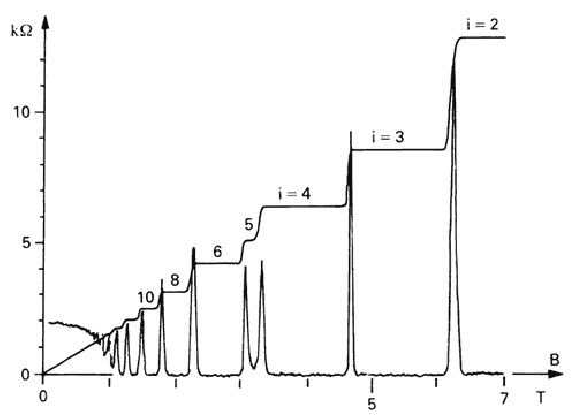
\includegraphics[width=\textwidth]{Figures/IntegerQHE.png}
			\caption{Integer quantum Hall effect (1980)}
		\end{subfigure}
		\hfill
		\begin{subfigure}[b]{0.4\textwidth}
			\centering
			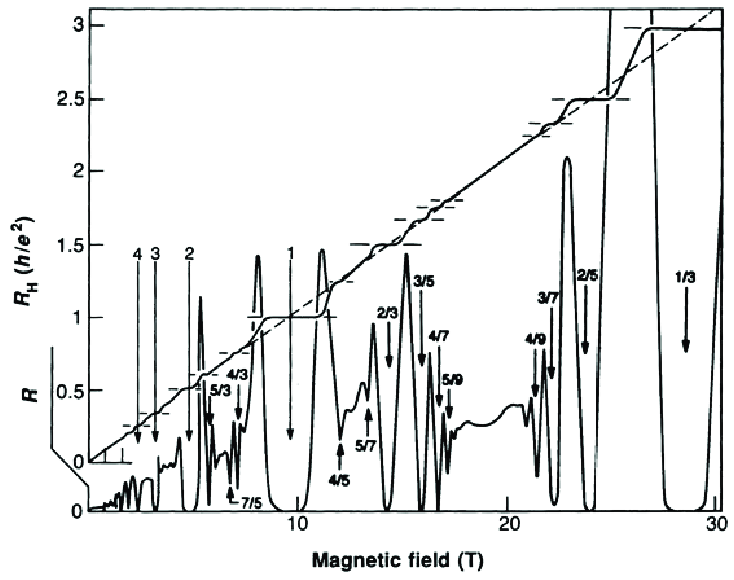
\includegraphics[width=\textwidth]{Figures/FractionalQHE.png}
			\caption{Fractional quantum Hall effect (1982)}
		\end{subfigure}
	\end{figure}
	have in common?
\end{frame}

\begin{frame}
	What do:
	\begin{figure}
		\centering
		\begin{subfigure}[b]{0.4\textwidth}
			\centering
			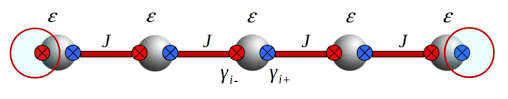
\includegraphics[width=\textwidth]{Figures/MajoranaEdgeModes.png}
			\caption{Majorana edge modes (not found yet)}
		\end{subfigure}
		\hfill
		\begin{subfigure}[b]{0.4\textwidth}
			\centering
			\includegraphics[width=\textwidth]{Figures/Fermi-Hubbard Ladders.pdf}
			\caption{Haldane phase (2021)}
		\end{subfigure}
	\end{figure}
	have in common?
\end{frame}

\begin{frame}{Unique gapped groundstates}
	\begin{columns}
		\begin{column}{0.7\textwidth}
			They are described by Hamiltonians $H$ that
			\begin{itemize}
				\item<2-> have a "unique gapped (bulk) ground-state" $\ket{\psi}$.
				\item<3-> are a sum of local therms.
			\end{itemize}
		\end{column}
		\begin{column}{0.3\textwidth}
			\begin{center}
				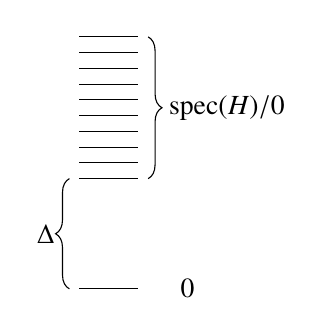
\begin{tikzpicture}
	\node (1L) at (0,0) {};
	\node (1R) at (1,0) {};
	\draw (1L) -- (1R);
	\foreach \i in {2,...,11}
	{
		\node (\i L) at (0,1+0.2*\i) {};
		\node (\i R) at (1,1+0.2*\i) {};
		\draw (\i L) -- (\i R);
	}
	\node[] (1Groundstate) at (1.5,0) {$0$};
	\draw [decorate,decoration={brace,amplitude=5pt},xshift=0cm,yshift=0pt] (0,0) -- (0,1.4) node [black,midway,xshift=-0.3cm] {$\Delta$};
	\draw [decorate,decoration={brace,amplitude=5pt},xshift=0cm,yshift=0pt] (1,1+0.2*11) -- (1,1.4)  node [black,midway,xshift=1cm] {$\textrm{spec}(H)/0$};
\end{tikzpicture}
			\end{center}
		\end{column}
	\end{columns}
	
\end{frame}

\begin{frame}{Gapped phases of quantum matter}
	Two Hamiltonians, $H(0)$ and $H(1)$ are connected if:
	\begin{center}
		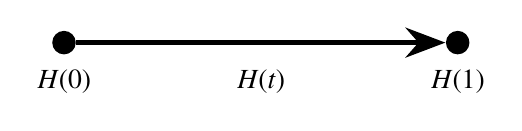
\begin{tikzpicture}
		\node (0) [circle,fill,inner sep=3pt] at (0,0) {};
		\node (0 -1) [] at (0,-0.5) {$H(0)$};
		\node (1) [circle,fill,inner sep=3pt] at (5,0) {};
		\node (1 -1) [] at (5,-0.5) {$H(1)$};
		\draw [line width=2pt,-{Stealth[scale = 1.2]}] (0) -- (1);
		\node (arrow) [] at (2.5,-0.5) {$H(t)$};
		\end{tikzpicture}
	\end{center}
	\begin{itemize}
		\item<2-> $H(t)$ is gapped.
		\item<3-> The local therms of $H(t)$ are continuous in $t$.
	\end{itemize}
	
\end{frame}

\begin{frame}
	Two states $\ket{\psi(0)}$ and $\ket{\psi(1)}$ are connected if
	\begin{center}
		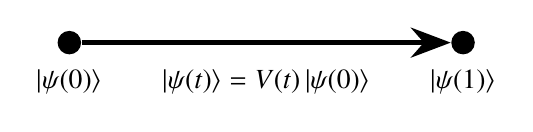
\begin{tikzpicture}
		\node (0) [circle,fill,inner sep=3pt] at (0,0) {};
		\node (0 -1) [] at (0,-0.5) {$\ket{\psi(0)}$};
		\node (1) [circle,fill,inner sep=3pt] at (5,0) {};
		\node (1 -1) [] at (5,-0.5) {$\ket{\psi(1)}$};
		\draw [line width=2pt,-{Stealth[scale = 1.2]}] (0) -- (1);
		\node (arrow) [] at (2.5,-0.5) {$\ket{\psi(t)}=V(t)\ket{\psi(0)}$};
		\end{tikzpicture}
	\end{center}
	\[V(t)=\mathcal{T}\exp(-i\int_0^t \d s K(s))\]
	is a locally generated family of unitaries (LGU).
\end{frame}

\begin{frame}
	These two concepts are equivalent:
	\begin{itemize}
		\item<2-> If $H(0)$ and $H(1)$ are equivalent through a path $H(t)$, the groundstates of $H(t)$ form a path.
		\item<3-> If $\ket{\psi(0)}$ and $\ket{\psi(1)}$ are equivalent through a path $\ket{\psi(t)}$, there exists a path of parent Hamiltonians $H(t)$ for $\ket{\psi(t)}$.
	\end{itemize}
\end{frame}

\begin{frame}{Gapped phases of quantum matter}
	\begin{center}
		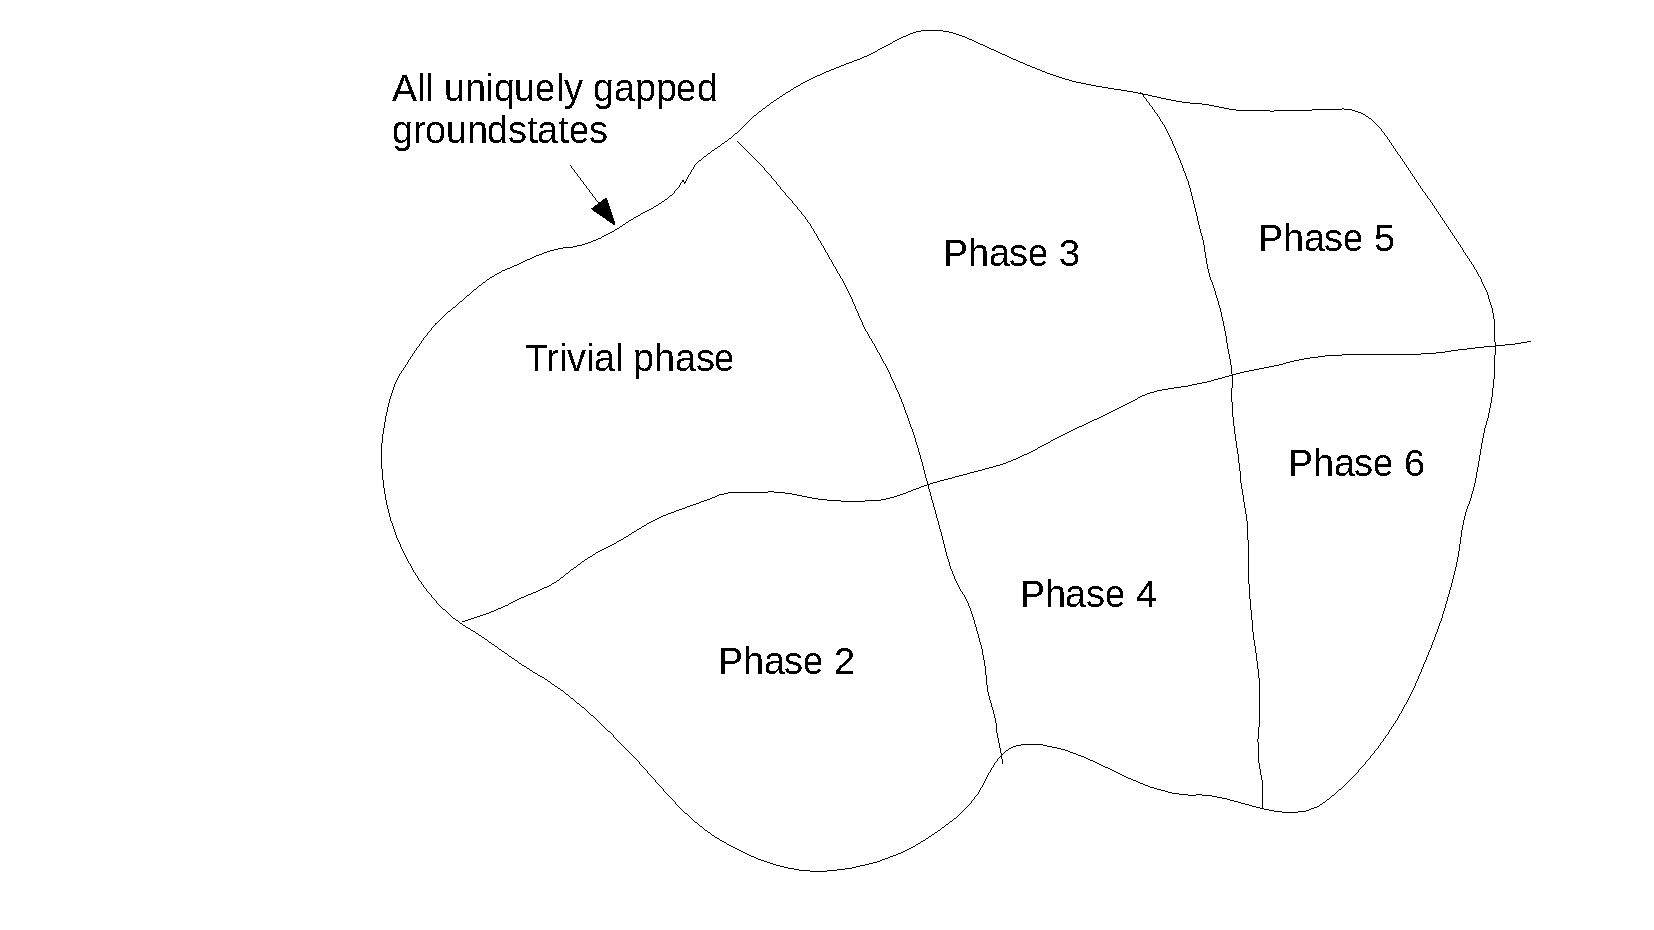
\includegraphics[trim={6cm 0 2.5cm 0},clip,width=0.8\textwidth]{Figures/GappedPhasesOfQuantumMatter.pdf}
	\end{center}
\end{frame}

\begin{frame}{Scope of this talk}
	\begin{center}
		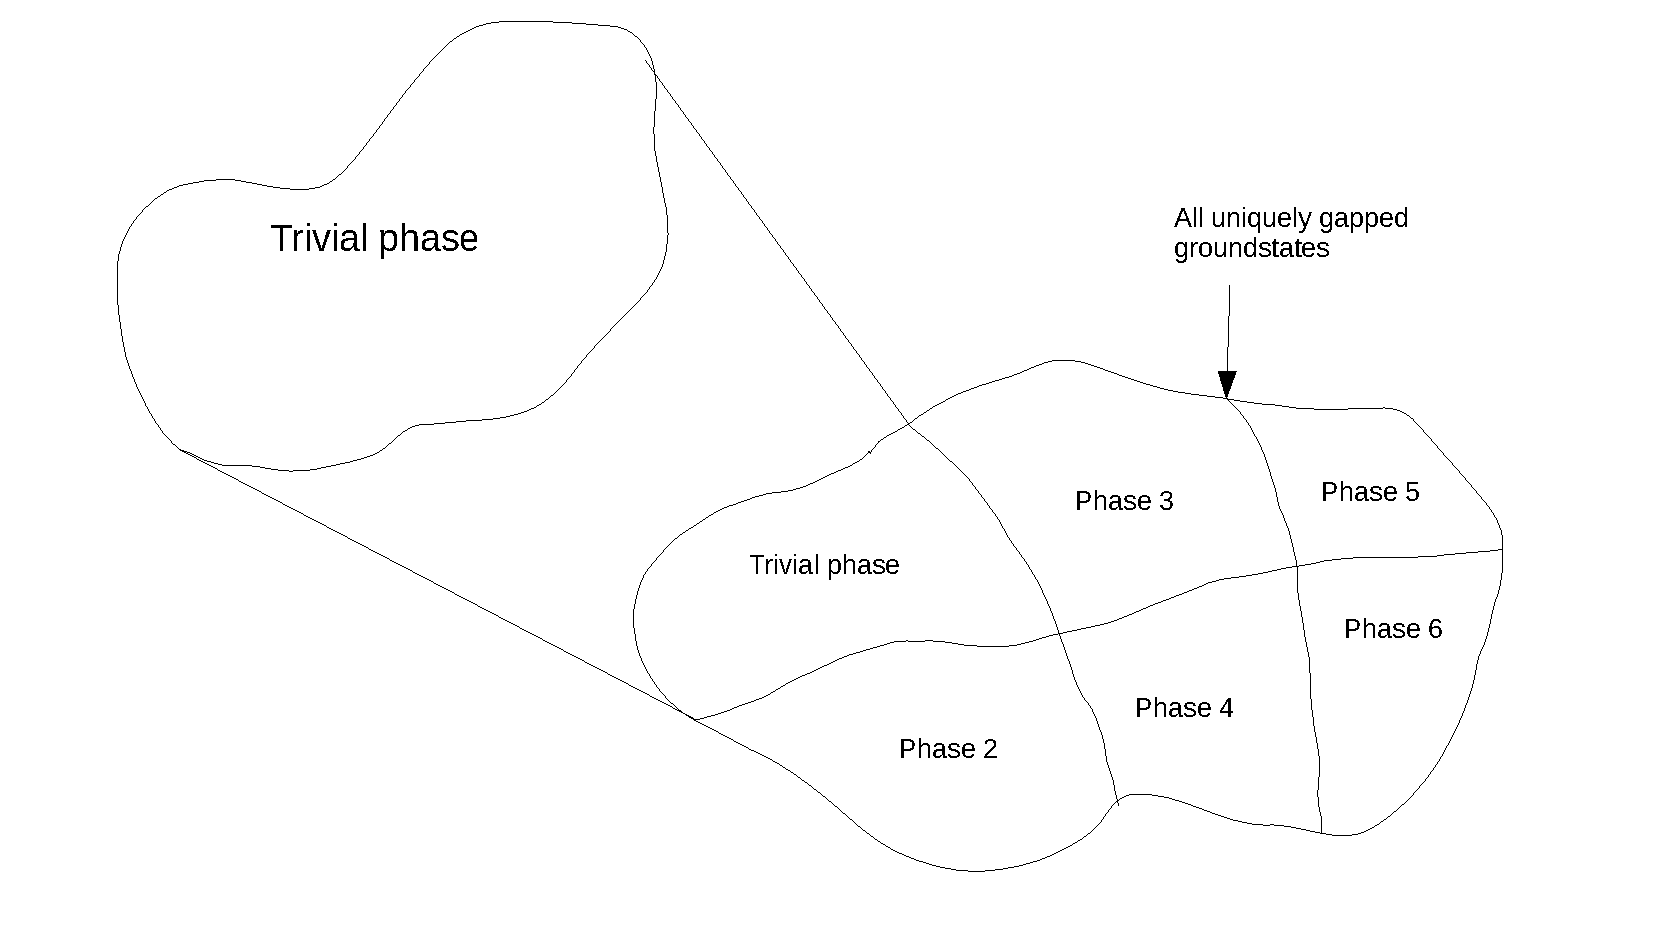
\includegraphics[trim={1.5cm 0 2cm 0},clip,width=0.8\textwidth]{Figures/TrivialGappedPhaseOfQuantumMatter.pdf}
	\end{center}
\end{frame}

\begin{frame}{The quantum lattice, $\Lambda$}
	\begin{center}
		\begin{tikzpicture}
	\foreach \i in {1,...,11}
	{
		\filldraw [black] (\i,0) circle (2pt);
		
	}
	\draw [decorate,decoration={brace,amplitude=5pt},xshift=0cm,yshift=0pt] (5+0.3,-0.3) -- (5-0.3,-0.3) node [black,midway,yshift=-0.3cm] {\footnotesize $\CC^d$};
\end{tikzpicture}
	\end{center}
\end{frame}

\begin{frame}{Trivial phase: short ranged entangled (SRE) phase}
	\begin{block}{Definition}
		$\ket{\psi}$ is SRE if:
		\[\ket{\phi}=V\ket{\psi}\]
		\begin{itemize}
			\item $V$, LGU.
			\item $\ket{\phi}$, product state.
		\end{itemize}
		\[\ket{\phi}=\bigotimes_{i\in\Lambda}\ket{v_i}\qquad \ket{v_i}\in\CC^d.\]
	\end{block}
\end{frame}

\begin{frame}{Trivial phase: SRE phase}
	\begin{center}
		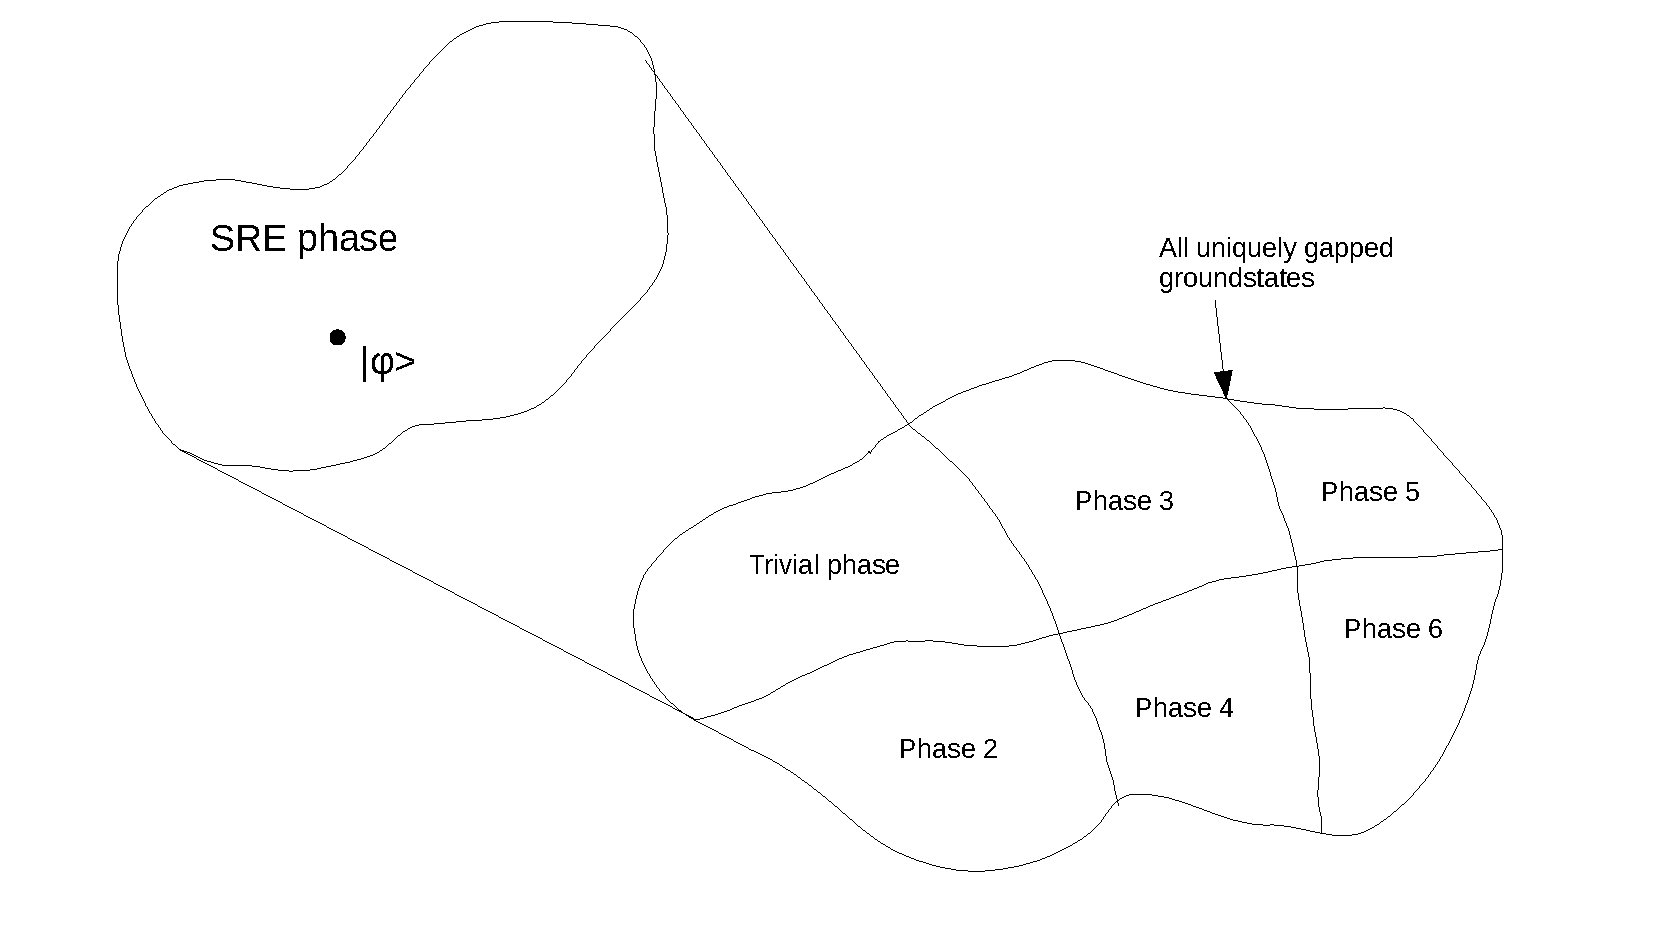
\includegraphics[trim={1.5cm 0 2cm 0},clip,width=0.8\textwidth]{Figures/SRE_Phase.pdf}
	\end{center}
\end{frame}

\begin{frame}{Example of LGU: Finite depth quantum cirquit}
	\begin{center}
		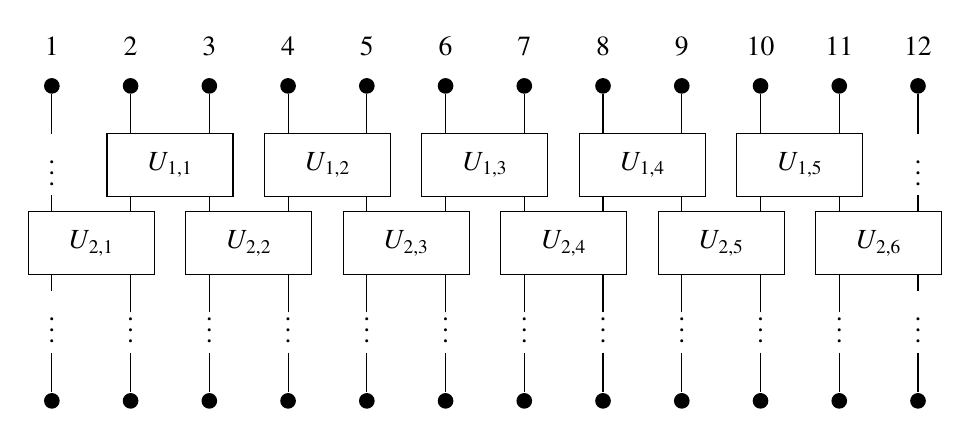
\begin{tikzpicture}
	\foreach \x in {0,...,11}{
		\node (-\x) [] at (\x,+0.5) {\pgfmathtruncatemacro\result{\x+1}\result};
		\node (\x) [circle,fill,inner sep=2pt] at (\x,0) {};
		\node (3\x) [circle,fill,inner sep=2pt] at (\x,-2) {};
		\node (4\x) [] at (\x,-3) {$\vdots$};
		\node (5\x) [circle,fill,inner sep=2pt] at (\x,-4) {};
	}
	
	\foreach \x in {1,...,10}{
		\node (2\x) [] at (\x,-3) {};
	}
	\node (20) at (0,-1) {$\vdots$};
	\node (211) at (11,-1) {$\vdots$};
	
	\foreach \x in {0,...,11}{
		\draw (\x) -- (2\x);
		\draw (2\x) -- (3\x);
		\draw (3\x) -- (4\x);
		\draw (4\x) -- (5\x);
	}
	
	\foreach \x in {1,...,5}
	\draw [fill=white] (2*\x-0.3-1,-0.6) rectangle (2*\x+0.3,-1.4);
	\foreach \x in {0,...,5}
	\draw [fill=white] (2*\x-0.3,-1.6) rectangle (2*\x+0.3+1,-2.4);
	
	\foreach \x in {1,...,5}
	\node [] at (2*\x-0.5,-1) {$U_{1,\x}$};
	\foreach \x in {0,...,5}
	\node [] at (2*\x+0.5,-2) {$U_{2,\pgfmathtruncatemacro\result{\x+1}\result}$};
	
	
\end{tikzpicture}
	\end{center}
\end{frame}

\begin{frame}{Finite depth quantum cirquit is locality preserving}
	\begin{center}
		\scalebox{0.75}{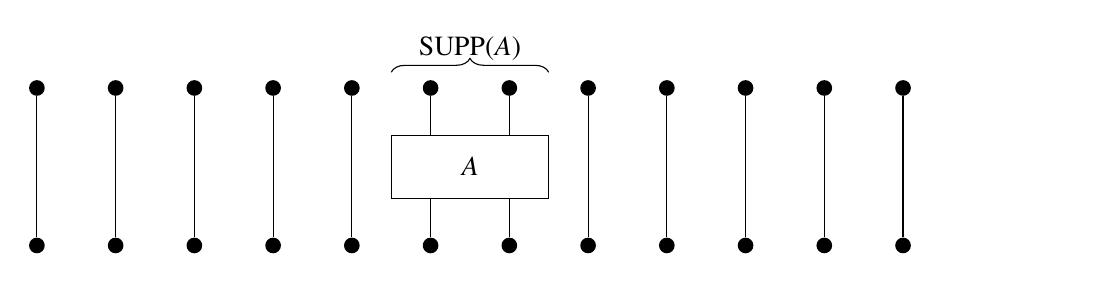
\begin{tikzpicture}
\foreach \x in {0,...,11}{
	\node (\x) [circle,fill,inner sep=2pt] at (\x,-1) {};
	\node (2\x) [] at (\x*1.2,-1) {};
	\node (3\x) [circle,fill,inner sep=2pt] at (\x,1) {};
	\draw (\x) -- (3\x);
}
\draw[fill=white] (4.5,0.4) rectangle (6.5,-0.4);
\node at (5.5,0) {$A$};
\draw [decorate,decoration={brace,amplitude=5pt},xshift=0cm,yshift=0pt] (4.5,1.2) -- (6.5,1.2) node [black,midway,yshift=0.3cm] {$\textrm{SUPP}(A)$};
\end{tikzpicture}}
	\end{center}
	\pause
	\begin{center}
		\scalebox{0.75}{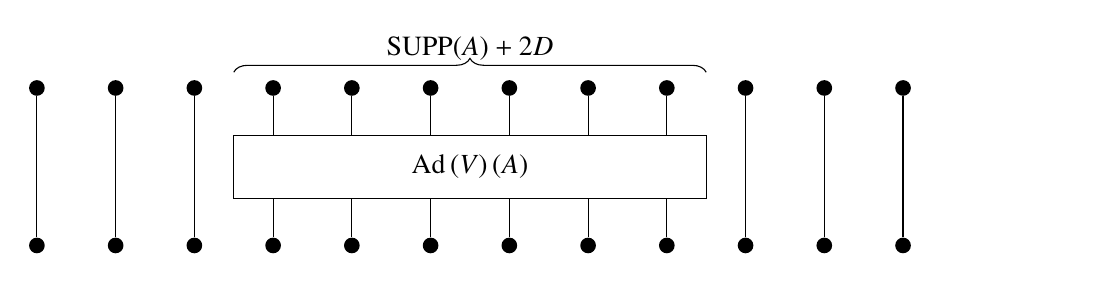
\begin{tikzpicture}
\foreach \x in {0,...,11}{
	\node (\x) [circle,fill,inner sep=2pt] at (\x,-1) {};
	\node (2\x) [] at (\x*1.2,-1) {};
	\node (3\x) [circle,fill,inner sep=2pt] at (\x,1) {};
	\draw (\x) -- (3\x);
}
\draw[fill=white] (2.5,0.4) rectangle (8.5,-0.4);
\node at (5.5,0) {$\Ad{V}(A)$};
\draw [decorate,decoration={brace,amplitude=5pt},xshift=0cm,yshift=0pt] (2.5,1.2) -- (8.5,1.2) node [black,midway,yshift=0.3cm] {$\textrm{SUPP}(A)+2D$};
\end{tikzpicture}}
	\end{center}
\end{frame}

\begin{frame}{Finite depth quantum cirquit is locality preserving}
	If I calculate $\Ad{V}(A)$ for $V$ a FDQC and $A$ local I only need unitaries in a cone:
	\begin{center}
		\scalebox{0.75}{
			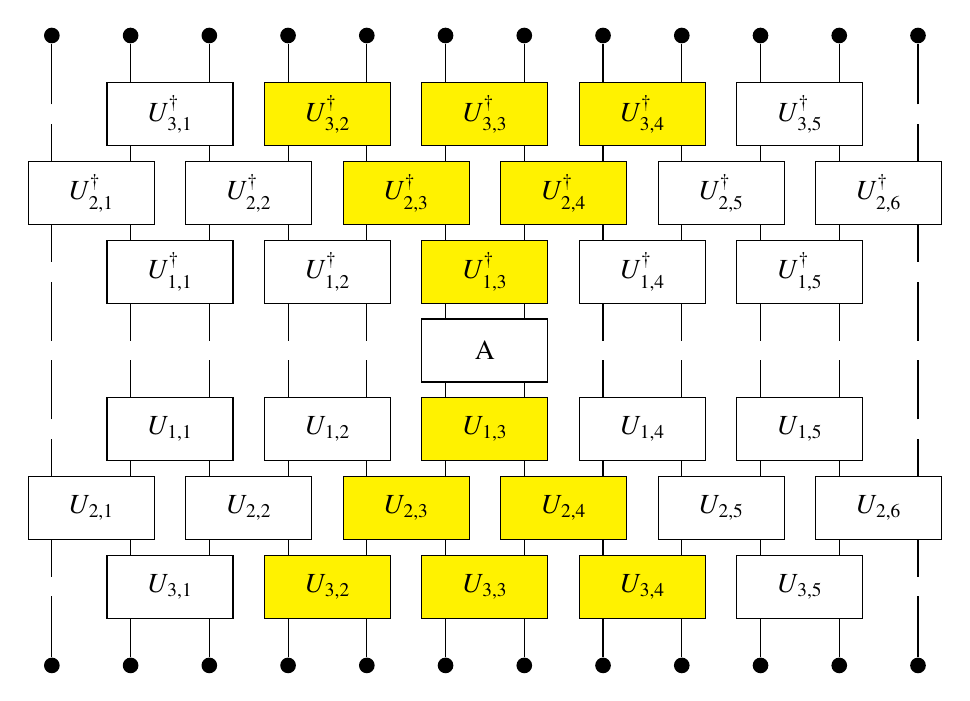
\begin{tikzpicture}
	\foreach \x in {0,...,11}{
		\foreach \y in {-4,...,4}{
			\ifthenelse{\y=-4 \OR \y=4}{\node (\y \x) [circle,fill,inner sep=2pt] at (\x,\y) {};}
			{\node (\y \x) [] at (\x,\y) {};}
		}
	}
	
	
	\foreach \x in {0,...,11}{
		\foreach \y in {-4,...,3}{
			\draw (\y \x) -- (\the\numexpr \y + 1\relax \x);
		}
	}

	\draw[fill=white] (4.7,0.4) rectangle (6.3,-0.4);
	\node at (5.5,0) {A};
	
	\foreach \x in {1,...,5}{
	\if\x3{
		\draw [fill=yellow] (2*\x-0.3-1,-0.6) rectangle (2*\x+0.3,-1.4);
		\draw [fill=yellow] (2*\x-0.3-1,0.6) rectangle (2*\x+0.3,1.4);
	}
	\else{
		\draw [fill=white] (2*\x-0.3-1,-0.6) rectangle (2*\x+0.3,-1.4);
		\draw [fill=white] (2*\x-0.3-1,0.6) rectangle (2*\x+0.3,1.4);
	}\fi};
	
	\foreach \x in {0,...,5}{
		\ifthenelse{\x=2 \OR \x=3}{\draw [fill=yellow] (2*\x-0.3,-1.6) rectangle (2*\x+0.3+1,-2.4);}{\draw [fill=white] (2*\x-0.3,-1.6) rectangle (2*\x+0.3+1,-2.4);}
		\ifthenelse{\x=2 \OR \x=3}{\draw [fill=yellow] (2*\x-0.3,1.6) rectangle (2*\x+0.3+1,2.4);}{\draw [fill=white] (2*\x-0.3,1.6) rectangle (2*\x+0.3+1,2.4);}
	};
	\foreach \x in {1,...,5}{
		\ifthenelse{\x=2 \OR \x=3 \OR \x=4}{\draw [fill=yellow] (2*\x-0.3-1,-2.6) rectangle (2*\x+0.3,-3.4);}{\draw [fill=white] (2*\x-0.3-1,-2.6) rectangle (2*\x+0.3,-3.4);}
		\ifthenelse{\x=2 \OR \x=3 \OR \x=4}{\draw [fill=yellow] (2*\x-0.3-1,2.6) rectangle (2*\x+0.3,3.4);}{\draw [fill=white] (2*\x-0.3-1,2.6) rectangle (2*\x+0.3,3.4);}
	}
	
	\foreach \x in {1,...,5}{
		\node [] at (2*\x-0.5,-1) {$U_{1,\x}$};
		\node [] at (2*\x-0.5,-3) {$U_{3,\x}$};
		\node [] at (2*\x-0.5,1) {$U_{1,\x}^\dagger$};
		\node [] at (2*\x-0.5,3) {$U_{3,\x}^\dagger$};
	}
	\foreach \x in {0,...,5}{
		\node [] at (2*\x+0.5,-2) {$U_{2,\the\numexpr \x + 1\relax}$};
		\node [] at (2*\x+0.5,2) {$U_{2,\the\numexpr \x + 1\relax}^\dagger$};
	}
	
	
\end{tikzpicture}

		}
	\end{center}
\end{frame}

\begin{frame}{Enriching with symmetry}
	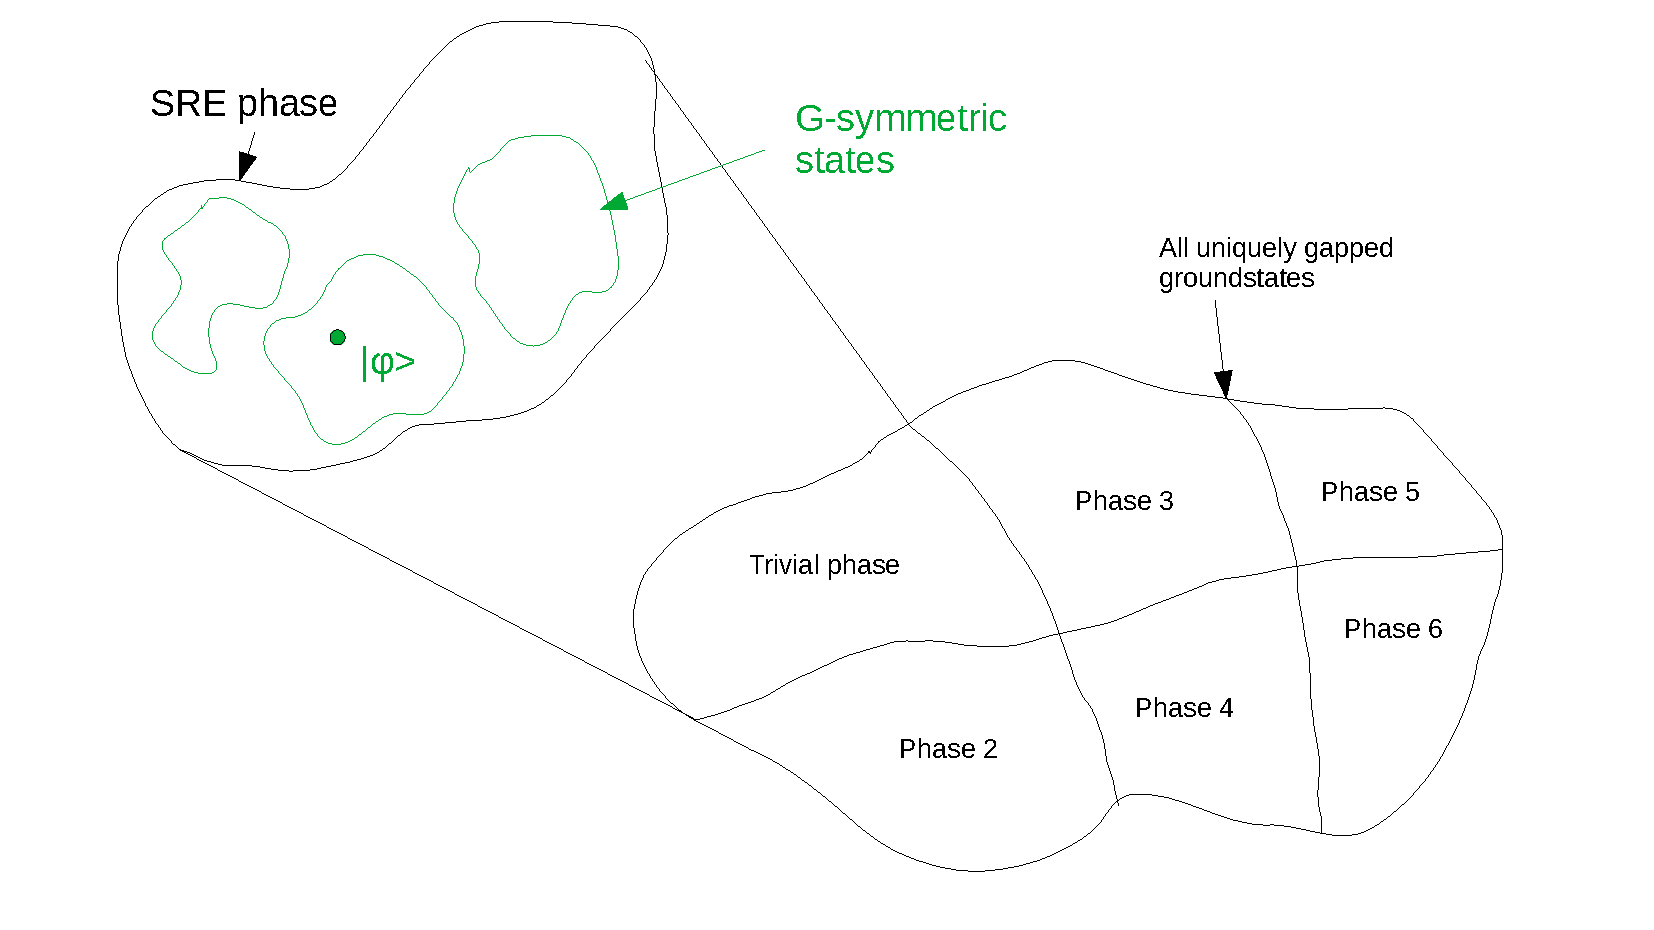
\includegraphics[width=\textwidth]{Figures/G-invariant_Parts_Of_SRE_Phase.pdf}
\end{frame}

\begin{frame}{Enriching with symmetry}
	\begin{center}
		\scalebox{0.75}{
		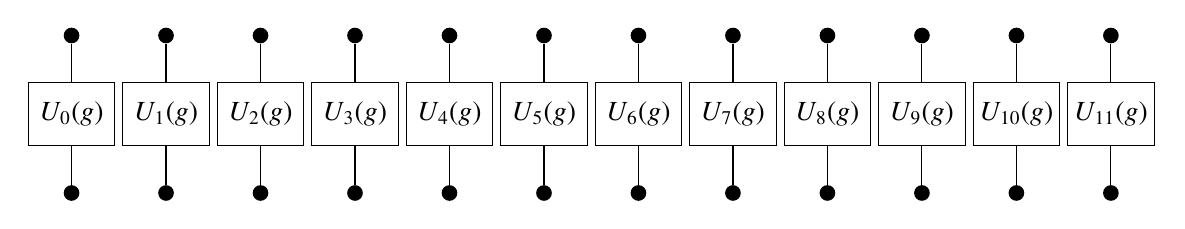
\begin{tikzpicture}
	\foreach \x in {0,...,11}{
		\node (\x) [circle,fill,inner sep=2pt] at (\x*1.2,0) {};
		\node (2\x) [] at (\x*1.2,-1) {};
		\node (3\x) [circle,fill,inner sep=2pt] at (\x*1.2,-2) {};
	}
	
	\foreach \x in {0,...,11}{
		\draw (\x) -- (2\x);
		\draw (2\x) -- (3\x);
	}
	
	\foreach \x in {0,...,11}
	\draw [fill=white] (\x*1.2-0.55,-0.6) rectangle (\x*1.2+0.55,-1.40);
	
	\foreach \x in {0,...,11}{
		\node (other \x) [] at (\x*1.2,-1) {$U_{\x}(g)$};
	}
\end{tikzpicture}
		}
	\end{center}
	\begin{itemize}
		\item $G$ compact Lie group.
		\item $U_i\in\hom(G,\UU(\CC^d))$ representation on on site Hilbert space.
		\item $U(g)=\bigotimes_{i\in\Lambda}U_i(g)$ group action.
	\end{itemize}
\end{frame}

\begin{frame}{Enriching with symmetry}
	\begin{itemize}
		\item<1-> $\ket{\psi}$ is $G$-invariant if
		\[U(g)\ket{\psi}=\ket{\psi}.\]
		\item<2-> An LGU,
		\[U(t)=\mathcal{T}\exp(-i\int_0^t \d s K(s))\]
		is $G$-invariant if each of the local therms of $K$ is $G$-invariant.
		\item<3-> In particular, a FDQC, $V$ is $G$-invariant if
		\[[U(g),V_{i,j}]=0.\]
	\end{itemize}
\end{frame}

\begin{frame}{SPT phases}
	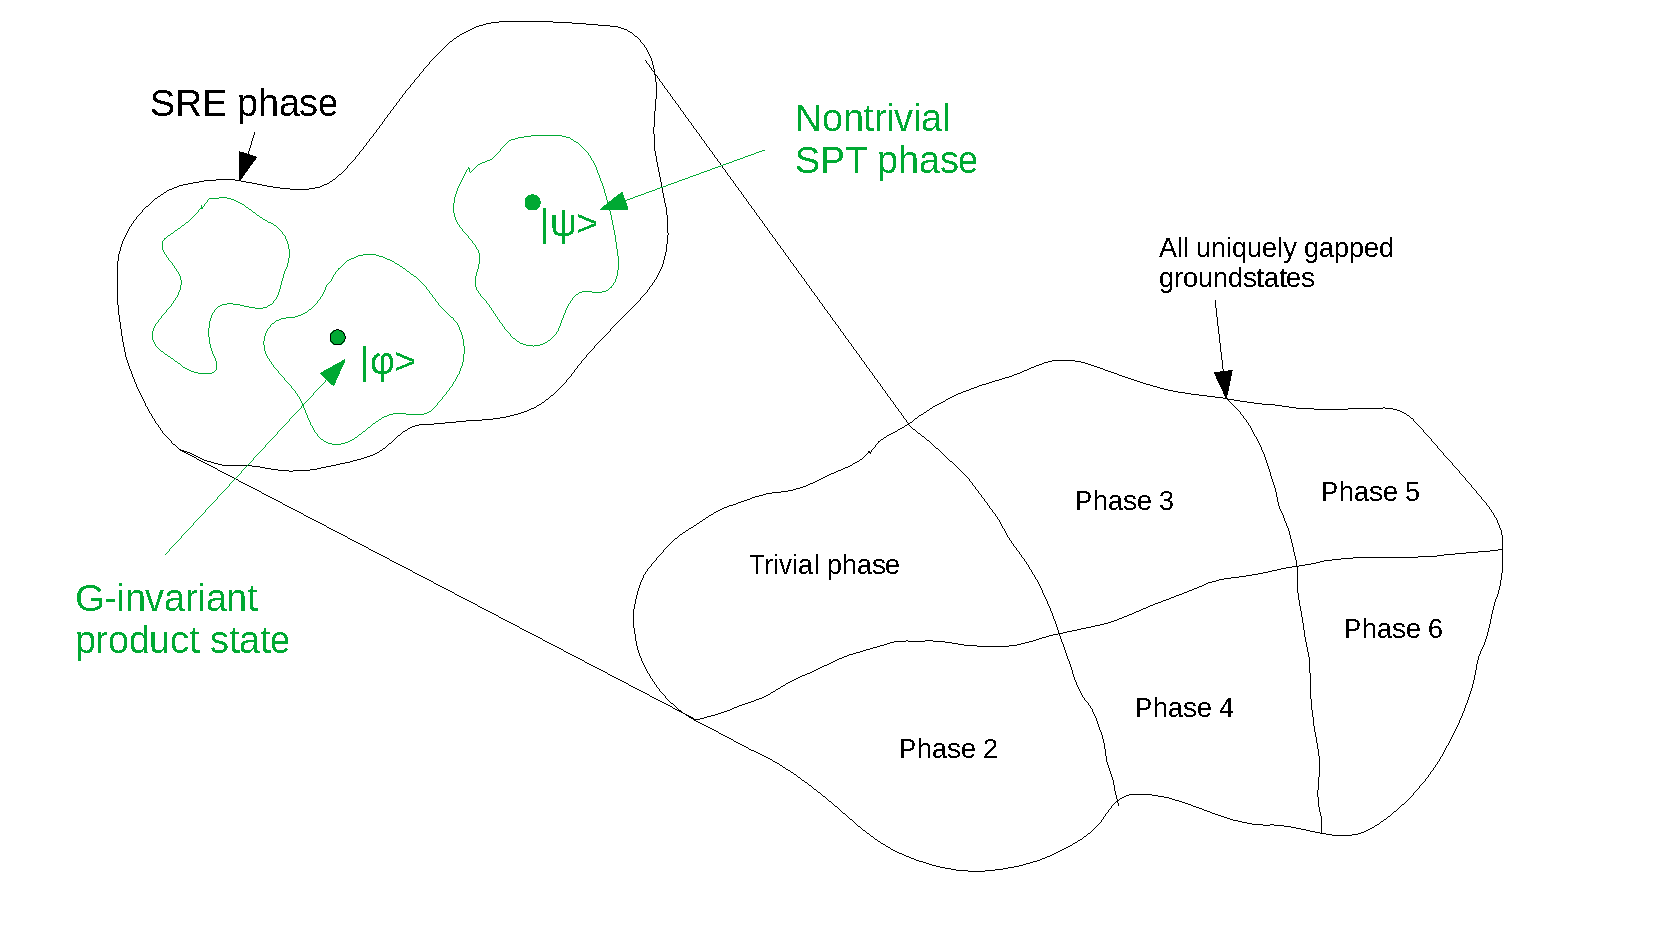
\includegraphics[width=\textwidth]{Figures/SPT_Phases.pdf}
\end{frame}

\begin{frame}{Example:}
	\begin{itemize}
		\item We take $G=\ZZ_2\times\ZZ_2$.
		\item We write the group elements as:
		\begin{align*}
			e&=(1,1)&g_x&=(-1,1)&g_y&=(1,-1)&g_z&=(-1,-1).
		\end{align*}
	\end{itemize}
	
\end{frame}

\begin{frame}{The singlet and the triplet}
	\begin{block}{On site Hilbert space}
		In $\CC^4\cong \CC^2\otimes \CC^2$, take as basis
		\begin{align*}
			&&\ket{s}&=\frac{1}{\sqrt{2}}(\ket{\uparrow\downarrow}-\ket{\downarrow\uparrow})&&\\
			\ket{0}&=\frac{1}{\sqrt{2}}(\ket{\uparrow\downarrow}+\ket{\downarrow\uparrow})&\ket{-1}&=\ket{\downarrow\downarrow}&\ket{1}&=\ket{\uparrow\uparrow}.
		\end{align*}
	\end{block}
	\pause
	\begin{block}{Group action}
		Take $U\in \textrm{Hom}(\ZZ^2\times \ZZ^2,U(\CC^4))$ by setting
		\begin{align*}
		U(-1,1)&=-\sigma_x\otimes \sigma_x&U(1,-1)&=-\sigma_y\otimes \sigma_y&U(-1,-1)&=-\sigma_z\otimes \sigma_z.
		\end{align*}
	\end{block}
\end{frame}

\begin{frame}{The singlet and the triplet}
	\begin{block}{Group action}
		Take $U\in \textrm{Hom}(\ZZ^2\times \ZZ^2,U(\CC^4))$ by setting
		\begin{align*}
		U(-1,1)&=-\sigma_x\otimes \sigma_x&U(1,-1)&=-\sigma_y\otimes \sigma_y&U(-1,-1)&=-\sigma_z\otimes \sigma_z.
		\end{align*}
	\end{block}
	Think of $\ZZ^2\times \ZZ^2$ as a subgroup of $SO(3)$ where
	\begin{itemize}
		\item $(-1,1)$ rotates around $x$-axis by $\pi$ radial.
		\item $(1,-1)$ rotates around $y$-axis by $\pi$ radial.
		\item $(-1,-1)$ rotates around $z$-axis by $\pi$ radial.
	\end{itemize}
	\pause
	\begin{block}{Back to the state}
		$\ket{s}$ is invariant under $\ZZ^2\times \ZZ^2$.\\
		$\ket{-1},\ket{0},\ket{1}$ transform irreducibly under $\ZZ^2\times \ZZ^2$.
	\end{block}
\end{frame}

\begin{frame}{Intermezzo linear and projective representations}
	We had a (linear) representation
	\begin{align*}
			U(-1,1)&=-\sigma_x\otimes \sigma_x&U(1,-1)&=-\sigma_y\otimes \sigma_y&U(-1,1)&=-\sigma_z\otimes \sigma_z.
	\end{align*}
	\pause
	I can rewrite this as:\\
	\begin{align*}
	U(-1,1)&=(i\sigma_x)\otimes (i\sigma_x)&U(1,-1)&=(i\sigma_y)\otimes (i\sigma_y)&U(-1,1)&=(i\sigma_z)\otimes (i\sigma_z).
	\end{align*}
	\pause
	Is
	\begin{align*}
		R(-1,1)&=i\sigma_x&R(1,-1)&=i\sigma_y&R(-1,-1)&=i\sigma_z
	\end{align*}
	 a representation on $\CC^2$? \pause No:
	\begin{equation*}
		R(-1,1)R(1,-1)=-R(1,-1)R(-1,1)=-i R(-1,-1).
	\end{equation*}
\end{frame}

\begin{frame}{The $G$-invariant product state}
	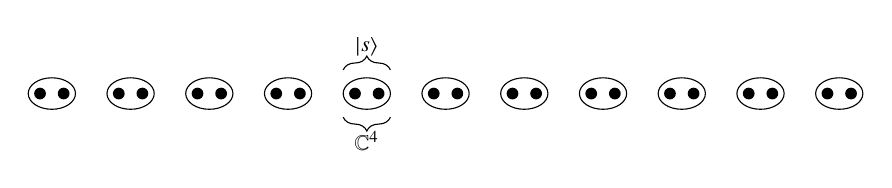
\begin{tikzpicture}
	\foreach \i in {1,...,11}
	{
		\draw[black] (\i,0) ellipse (0.3 and 0.2);
		\node (\i L) [circle,fill,inner sep=1.5pt] at (\i-0.15,0) {};
		\node (\i R) [circle,fill,inner sep=1.5pt] at (\i+0.15,0) {};
		
	}
	\draw [decorate,decoration={brace,amplitude=5pt},xshift=0cm,yshift=0pt] (5-0.3,0.3) -- (5+0.3,0.3) node [black,midway,yshift=0.3cm] {\footnotesize $\ket{s}$};
	\draw [decorate,decoration={brace,amplitude=5pt},xshift=0cm,yshift=0pt] (5+0.3,-0.3) -- (5-0.3,-0.3) node [black,midway,yshift=-0.3cm] {\footnotesize $\CC^4$};
	
\end{tikzpicture}\\
	On $\bigotimes_{i\in\Lambda}(\CC^4)$, define a state
	\begin{equation*}
		\ket{\phi}=\bigotimes_{i\in\Lambda}\ket{s}_{(i,L),(i,R)}
	\end{equation*}
	\pause
	It is a $G$-invariant product state.
\end{frame}

\begin{frame}{The entangled pair state}
	\begin{tikzpicture}
	\foreach \i in {1,...,10}
	{
		\draw[black] (\i+0.5,0) ellipse (0.48 and 0.2);
		\filldraw [black] (\i-0.15,0) circle (2pt);
		\filldraw [black] (\i+0.15,0) circle (2pt);
	}
	\filldraw [black] (11-0.15,0) circle (2pt);
	\filldraw [black] (11+0.15,0) circle (2pt);
	\draw [decorate,decoration={brace,amplitude=5pt},xshift=0cm,yshift=0pt] (5,0.3) -- (5+1,0.3) node [black,midway,yshift=0.3cm] {\footnotesize $\ket{s}$};
	\draw [decorate,decoration={brace,amplitude=5pt},xshift=0cm,yshift=0pt] (5+0.3,-0.3) -- (5-0.3,-0.3) node [black,midway,yshift=-0.3cm] {\footnotesize $\CC^4$};
	\begin{scope}
		\clip(0.5,0.2)rectangle(1,-0.2);
		\draw[black] (0.5,0) ellipse (0.48 and 0.2);
	\end{scope}
	\begin{scope}
		\clip(11,0.2)rectangle(11.5,-0.2);
		\draw[black] (11.5,0) ellipse (0.48 and 0.2);
	\end{scope}
	\node (iL) [] at (5.5,-1) {$(i,L)$};
	\draw[black,->] (6L) -- (iL);
	\node (iR) [] at (6.5,-1) {$(i,R)$};
	\draw[black,->] (6R) -- (iR);
\end{tikzpicture}\\
	On $\bigotimes_{i\in\Lambda}(\CC^4)$, define a state
	\begin{equation*}
		\ket{\psi}=\bigotimes_{i\in\Lambda}\ket{s}_{(i,R),(i+1,L)}
	\end{equation*}
	\pause
	It is $G$-invariant.
\end{frame}


\begin{frame}{Connecting $\ket{\psi}$ and $\ket{\phi}$}
	I can connect $\ket{\psi}$ and $\ket{\phi}$ with a quantum circuit of depth 3:
	\begin{center}
		\scalebox{0.75}{
		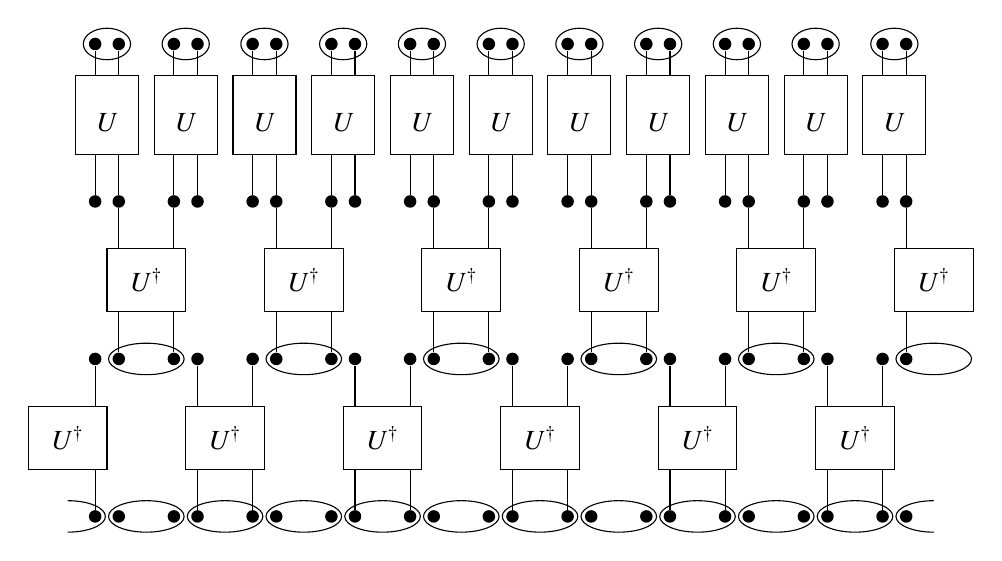
\begin{tikzpicture}
		\foreach \i in {1,...,11}
	{
		\draw[black] (\i,0) ellipse (0.3 and 0.2);
		\foreach \j in {0,...,3}{
			\node (Left\i\j) [circle,fill,inner sep=1.6pt] at (\i-0.15,-2*\j) {};
			\node (Right\i\j) [circle,fill,inner sep=1.6pt] at (\i+0.15,-2*\j) {};
		}
	}
	\newcommand\y{6}
	
	\foreach \i in {1,...,10}
	{
		\draw[black] (\i+0.5,-\y) ellipse (0.48 and 0.2);
	}
	\begin{scope}
		\clip(0.5,-\y+0.2)rectangle(1,-\y-0.2);
		\draw[black] (0.5,-\y) ellipse (0.48 and 0.2);
	\end{scope}
	\begin{scope}
		\clip(11,-\y+0.2)rectangle(11.5,-\y-0.2);
		\draw[black] (11.5,-\y) ellipse (0.48 and 0.2);
	\end{scope}

	\foreach \i in {1,...,11}
	{
		\draw (Left\i0) -- (Left\i1);
		\draw (Right\i0) -- (Right\i1);
		\ifthenelse{\isodd{\i}}{
			\draw (Right\i1) -- (Right\i2);
			\draw (Left\i2) -- (Left\i3);
		}{
			\draw (Left\i1) -- (Left\i2);
			\draw (Right\i2) -- (Right\i3);
		}
	}
	\foreach \i in {1,...,11}{
		\draw[fill=white] (\i-0.4,-0.4) rectangle (\i+0.4,-1.4);
		\node[] (\i) at (\i,-1) {$U$};
		\ifthenelse{\isodd{\i}}{
			\draw[fill=white] (\i,-2.6) rectangle (\i+1,-3.4);
			\node[] (SecondUnitary\i) at (\i+0.5,-3) {$U^\dagger$};
			\draw[fill=white] (\i-1,-4.6) rectangle (\i,-5.4);
			\node[] (ThirdUnitary\i) at (\i-0.5,-5) {$U^\dagger$};
			\draw[black] (\i+0.5,-4) ellipse (0.48 and 0.2);
		}{}
	}
\end{tikzpicture}
		}
	\end{center}
	\pause
	However, this is not $G$-invariant.\\
	\pause
	Can I find a $G$-invariant quantum cirquit?
\end{frame}

\begin{frame}{The entangled pair state}
	$\ket{\psi}=\ket{\psi_L}\otimes\ket{s}\otimes\ket{\psi_R}$ \\
	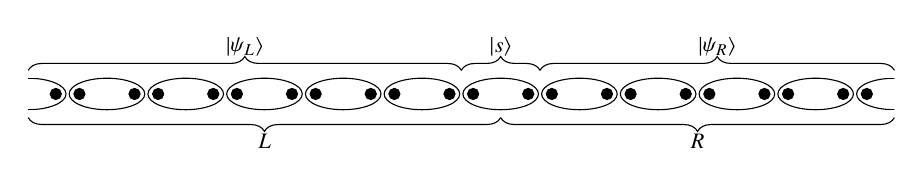
\begin{tikzpicture}
	\foreach \i in {1,...,10}
	{
		\draw[black] (\i+0.5,0) ellipse (0.48 and 0.2);
		\filldraw [black] (\i-0.15,0) circle (2pt);
		\filldraw [black] (\i+0.15,0) circle (2pt);
		
	}
	\filldraw [black] (11-0.15,0) circle (2pt);
	\filldraw [black] (11+0.15,0) circle (2pt);
	\begin{scope}
		\clip(0.5,0.2)rectangle(1,-0.2);
		\draw[black] (0.5,0) ellipse (0.48 and 0.2);
	\end{scope}
	\begin{scope}
		\clip(11,0.2)rectangle(11.5,-0.2);
		\draw[black] (11.5,0) ellipse (0.48 and 0.2);
	\end{scope}
	\draw [decorate,decoration={brace,amplitude=5pt},xshift=0cm,yshift=0pt] (7,0.3) -- (11.5,0.3) node [black,midway,yshift=0.3cm] {\footnotesize $\ket{\psi_R}$};
	\draw [decorate,decoration={brace,amplitude=5pt},xshift=0cm,yshift=0pt] (0.5,0.3) -- (6,0.3) node [black,midway,yshift=0.3cm] {\footnotesize $\ket{\psi_L}$};
	\draw [decorate,decoration={brace,amplitude=5pt},xshift=0cm,yshift=0pt] (6,0.3) -- (7,0.3) node [black,midway,yshift=0.3cm] {\footnotesize $\ket{s}$};
	\draw [decorate,decoration={brace,amplitude=5pt},xshift=0cm,yshift=0pt] (6.5,-0.3) -- (0.5,-0.3)  node [black,midway,yshift=-0.3cm] {\footnotesize $L$};
	\draw [decorate,decoration={brace,amplitude=5pt},xshift=0cm,yshift=0pt] (11.5,-0.3) -- (6.5,-0.3)  node [black,midway,yshift=-0.3cm] {\footnotesize $R$};
\end{tikzpicture}\\
	\pause
	\begin{equation*}
		\textrm{Tr}_L(\ket{\psi}\bra{\psi})=\frac{1}{2}(\ket{\uparrow}\bra{\uparrow}+\ket{\downarrow}\bra{\downarrow})\otimes\ket{\psi_R}\bra{\psi_R}.
	\end{equation*}
	This is a (perfectly) mixed state. Take a basis of this mixed state
	\begin{align*}
		\ket{v_1}=&\ket{\uparrow}\otimes\ket{\psi_R}&\ket{v_2}=&\ket{\downarrow}\otimes\ket{\psi_R}.
	\end{align*}
	\pause
	This subspace transforms under $\ZZ_2\times\ZZ_2$ as
	\begin{align*}
		R(-1,1)&=i\sigma_x&R(1,-1)&=i\sigma_y&R(-1,-1)&=i\sigma_z.
	\end{align*}
	\begin{block}{Claim}
		The right half of this chain transforms projectively under the group action.
	\end{block}
\end{frame}

\begin{frame}{The product state}
	$\ket{\phi}=\ket{\phi_{L}}\otimes\ket{\phi_{R}}$ \\
	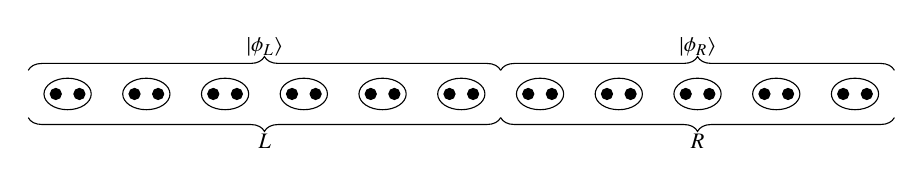
\begin{tikzpicture}
	\foreach \i in {1,...,11}
	{
		\draw[black] (\i,0) ellipse (0.3 and 0.2);
		\filldraw [black] (\i-0.15,0) circle (2pt);
		\filldraw [black] (\i+0.15,0) circle (2pt);
		
	}
	\draw [decorate,decoration={brace,amplitude=5pt},xshift=0cm,yshift=0pt] (6.5,0.3) -- (11.5,0.3) node [black,midway,yshift=0.3cm] {\footnotesize $\ket{\phi_{R}}$};
	\draw [decorate,decoration={brace,amplitude=5pt},xshift=0cm,yshift=0pt] (0.5,0.3) -- (6.5,0.3) node [black,midway,yshift=0.3cm] {\footnotesize $\ket{\phi_{L}}$};
	\draw [decorate,decoration={brace,amplitude=5pt},xshift=0cm,yshift=0pt] (6.5,-0.3) -- (0.5,-0.3)  node [black,midway,yshift=-0.3cm] {\footnotesize $L$};
	\draw [decorate,decoration={brace,amplitude=5pt},xshift=0cm,yshift=0pt] (11.5,-0.3) -- (6.5,-0.3)  node [black,midway,yshift=-0.3cm] {\footnotesize $R$};
\end{tikzpicture}\\
	\pause
	\begin{equation*}
		\textrm{Tr}_L(\ket{\phi}\bra{\phi})=\ket{\phi_{R}}\bra{\phi_{R}}.
	\end{equation*}
	\pause
	This subspace transforms under $\ZZ_2\times\ZZ_2$ one dimensionally.
	\begin{block}{Claim}
		The right half of this chain transforms linearly under the group action.
	\end{block}
\end{frame}

\begin{frame}{Proof that I can't connect $\ket{\phi}$ and $\ket{\psi}$ through finite depth quantum cirquit}
	Suppose I can connect $\ket{\psi}$ and $\ket{\phi}$ through $G$-invariant quantum cirquit of depth $d$:
	\begin{figure}
		\center
		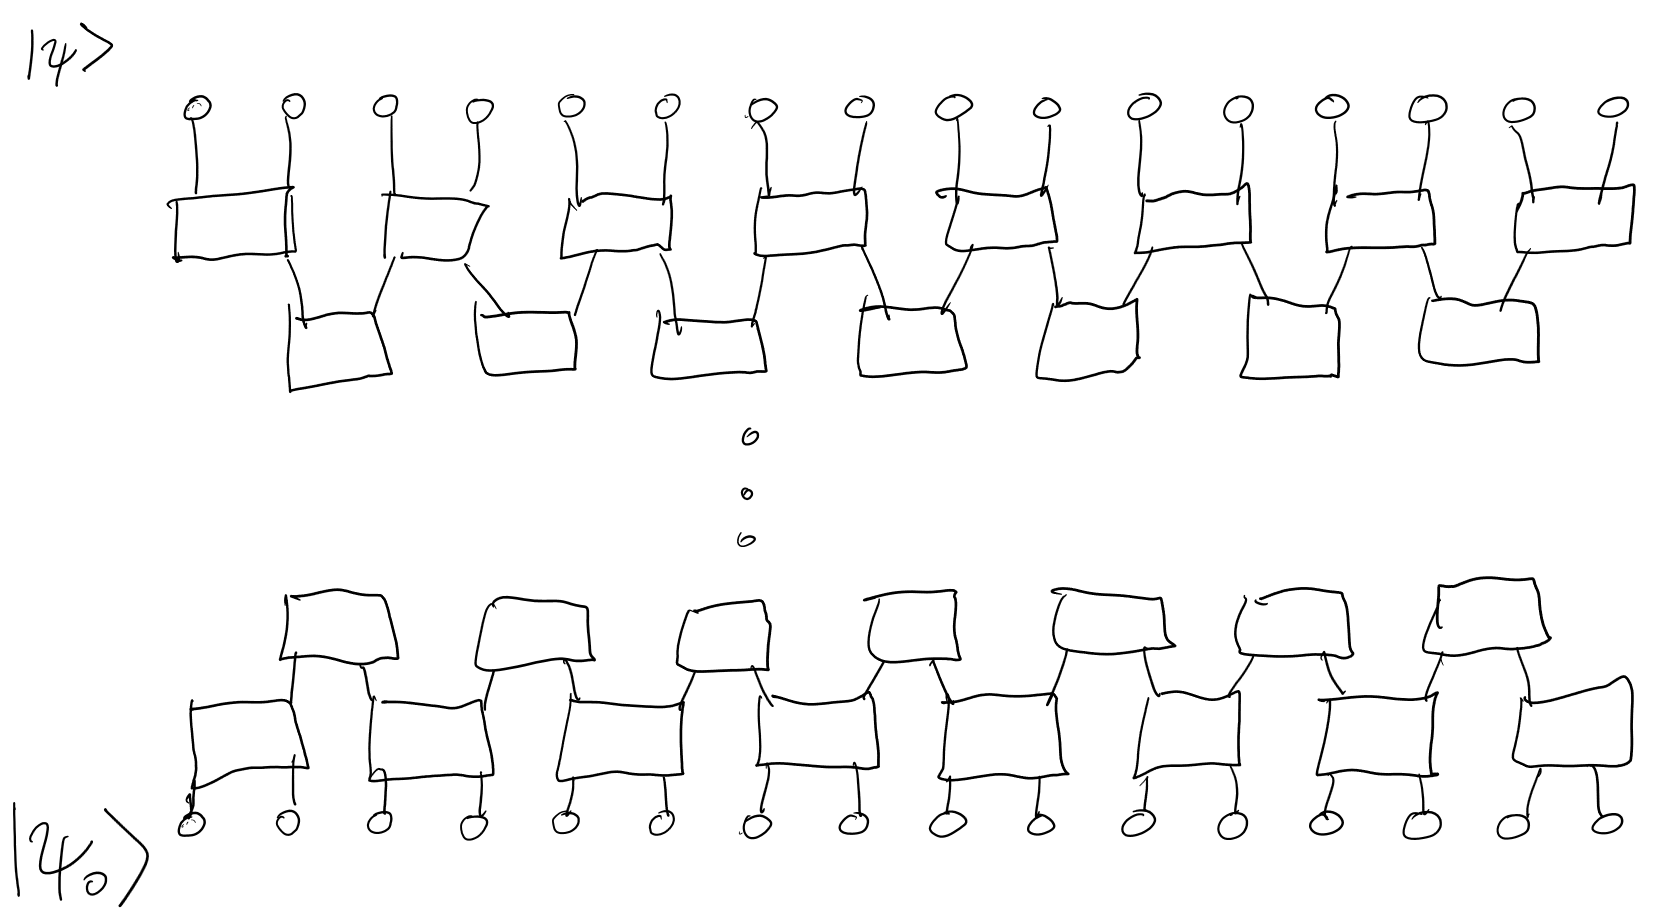
\includegraphics[width=0.8\textwidth]{Figures/ConnectingPsiAndPsi0Proof.png}
	\end{figure}
\end{frame}

\begin{frame}{Proof that I can't connect $\ket{\phi}$ and $\ket{\psi}$ through finite depth quantum cirquit}
	Set all unitaries of FDQC with support on the left to be $\id$.
	\begin{figure}
		\center
		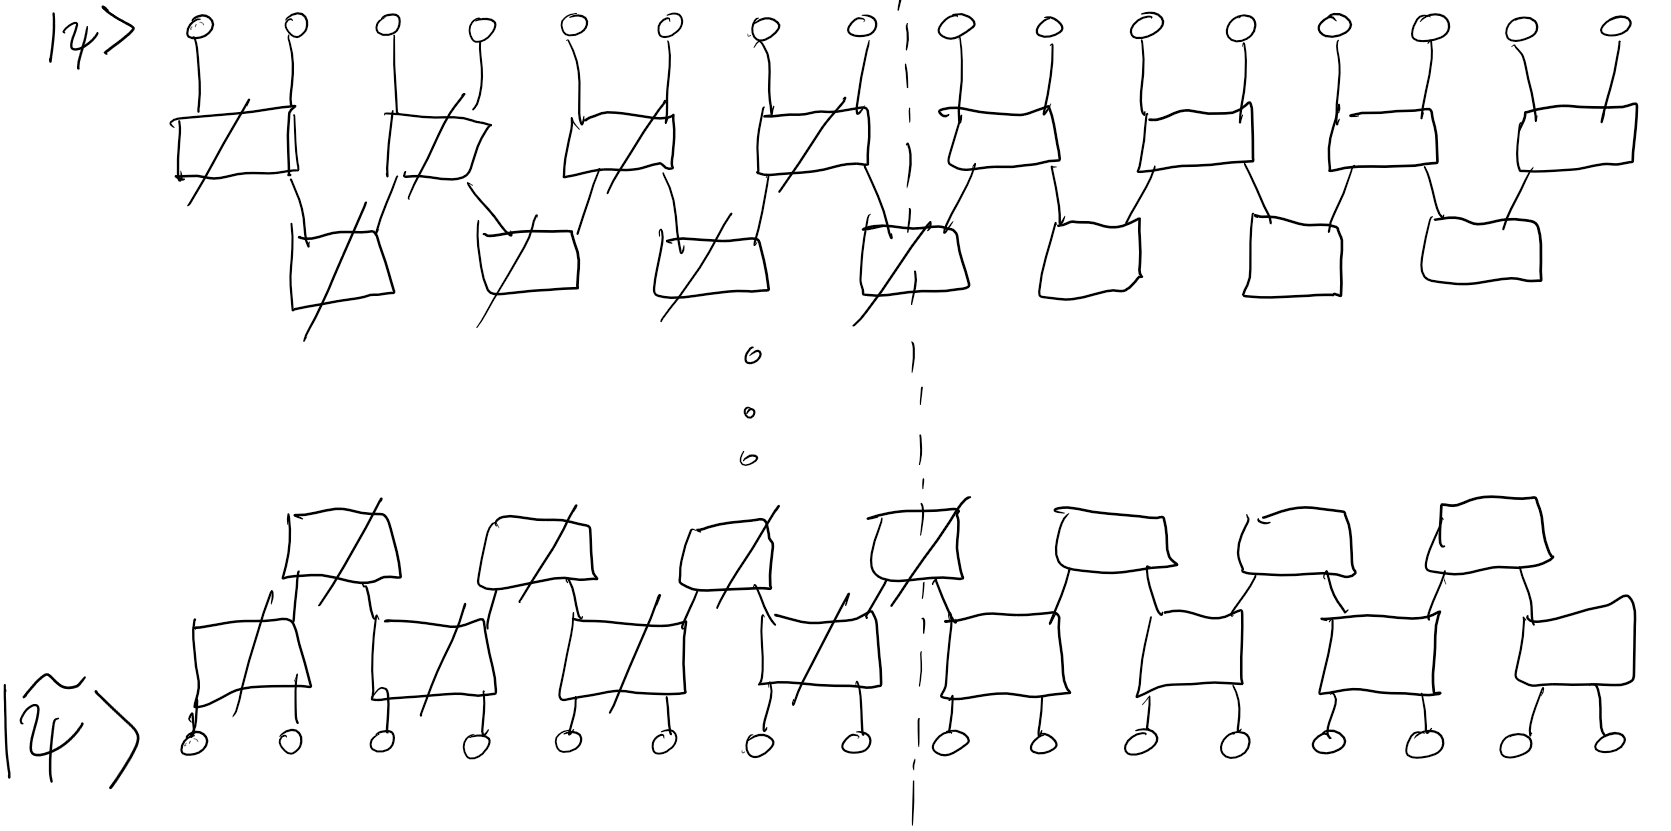
\includegraphics[width=0.75\textwidth]{Figures/ConnectingPsiAndPsi0Proof2.png}
	\end{figure}
\end{frame}

\begin{frame}{Proof that I can't connect $\ket{\phi}$ and $\ket{\psi}$ through finite depth quantum cirquit}
	This implies that there exists a state $\ket{\tilde\psi}$ that looks like $\ket{\psi}$ on the left and $\ket{\phi}$ on the right:
	\begin{figure}
		\center
		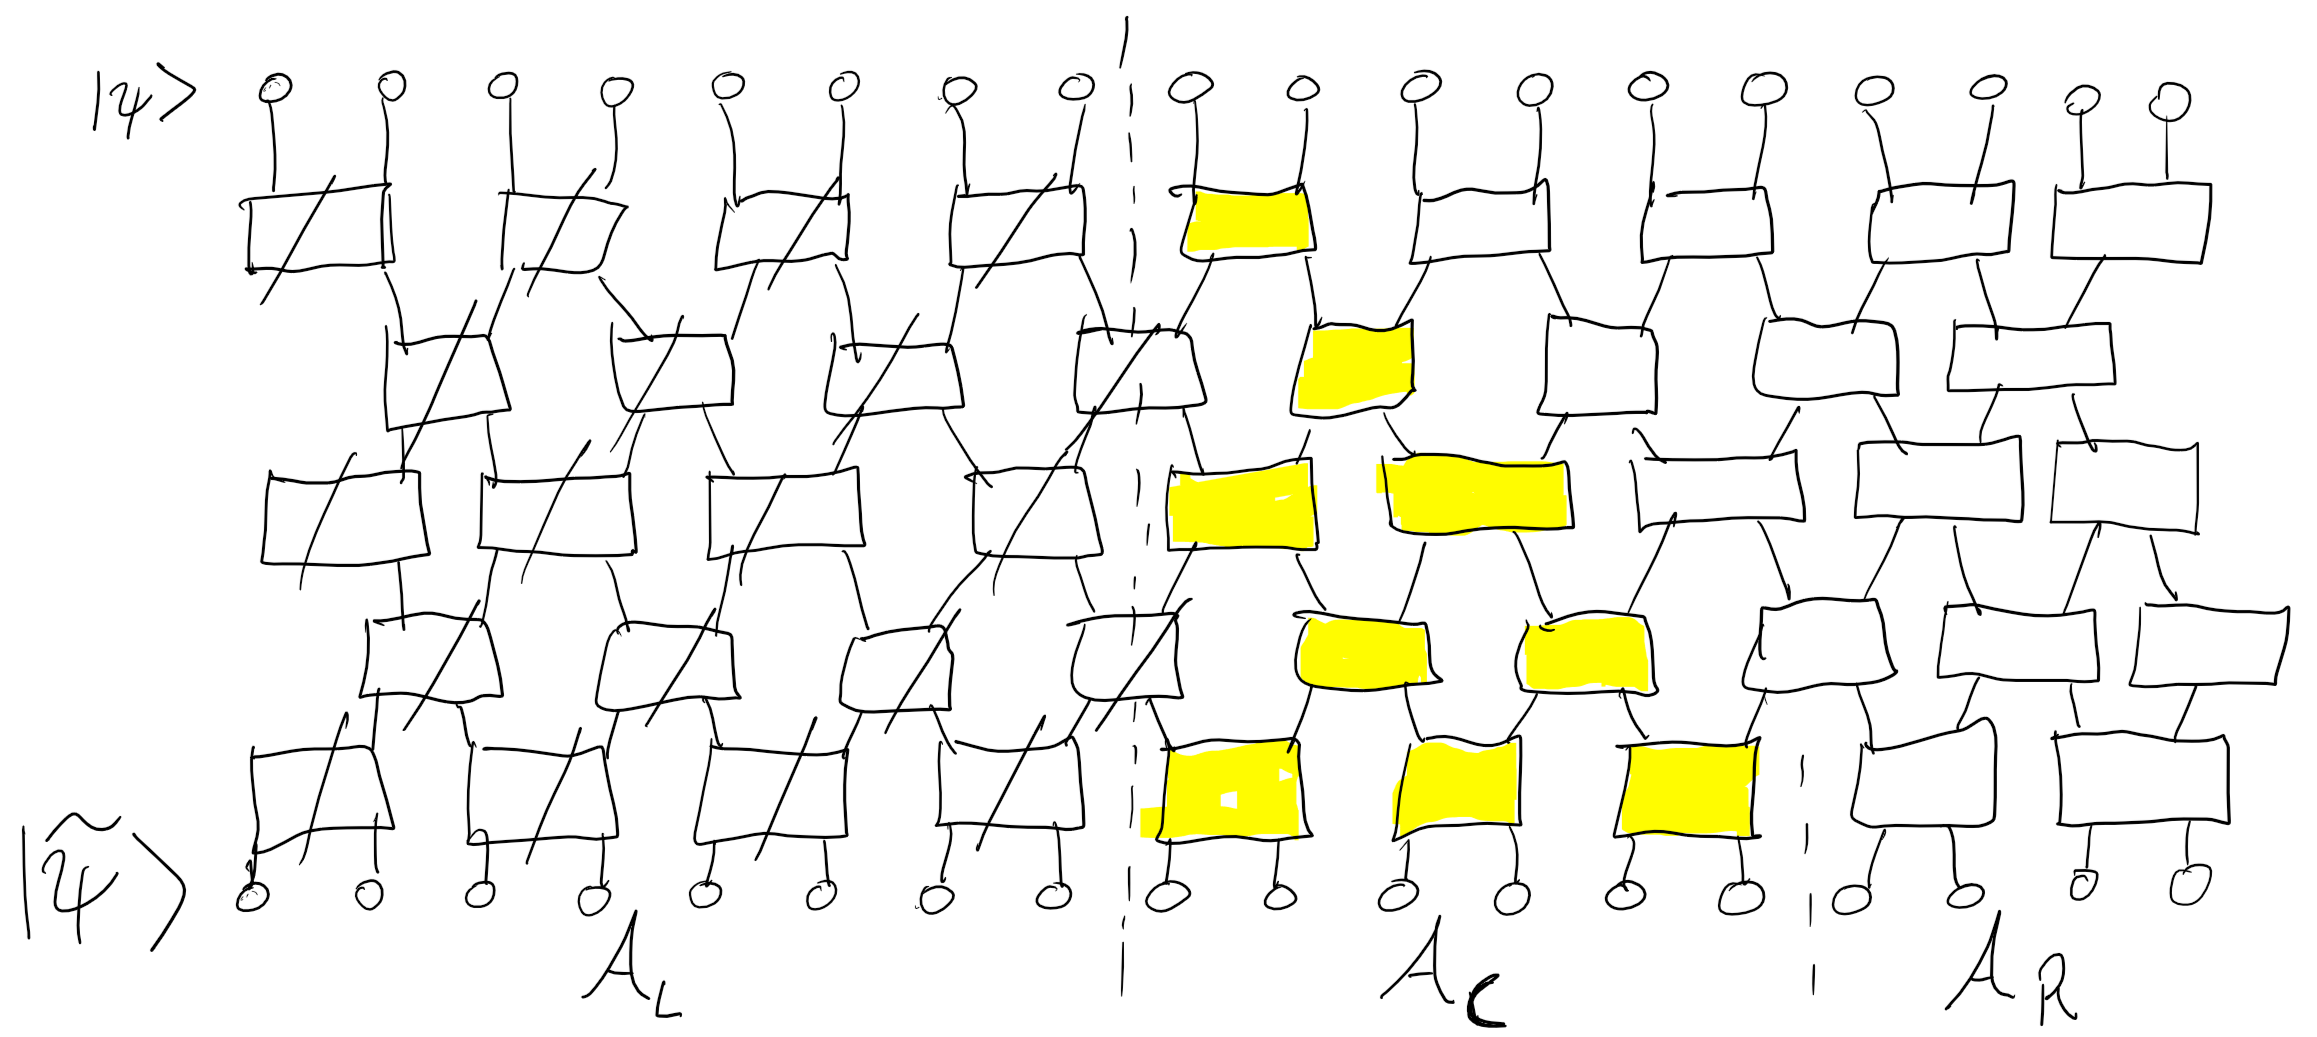
\includegraphics[width=0.75\textwidth]{Figures/ConnectingPsiAndPsi0Proof2_WithLightcone.png}
	\end{figure}
	\pause
	For $A_L\in\AA_L$ and $A_R\in\AA_R$ respectively I have
	\begin{align}
		\bra{\tilde\psi}A_L\ket{\tilde{\psi}}&=\bra{\psi}A_L\ket{\psi}&\bra{\tilde\psi}A_R\ket{\tilde{\psi}}&=\bra{\phi}A_R\ket{\phi}.
	\end{align}
\end{frame}

\begin{frame}{Proof that I can't connect $\ket{\phi}$ and $\ket{\psi}$ through finite depth quantum cirquit}
	For $A_L\in\AA_L$ and $A_R\in\AA_R$ respectively I have
	\begin{align}
		\bra{\tilde\psi}A_L\ket{\tilde{\psi}}&=\bra{\psi}A_L\ket{\psi}&\bra{\tilde\psi}A_R\ket{\tilde{\psi}}&=\bra{\phi}A_R\ket{\phi}.
	\end{align}
	\pause
	This means that
	\begin{itemize}
		\item $\ket{\tilde{\psi}}$ transforms projectively under $U_L(g)=\bigotimes_{i \in L}U_i(g)$.
		\item $\ket{\tilde{\psi}}$ transforms trivially under $U_R(g)=\bigotimes_{i \in R}U_i(g)$.
		\item <3->$U_C(g)=\bigotimes_{i\in C}U_i(g)$ is a linear representation.
	\end{itemize}
	\pause
	\pause
	$\ket{\tilde{\psi}}$ has to transform projectively\\
	\pause
	$\Rightarrow$ $\ket{\tilde{\psi}}$ cannot be $G$-invariant.
\end{frame}

\begin{frame}{SP phases in 1d for $G=\ZZ_2\times \ZZ_2$}
	\begin{center}
		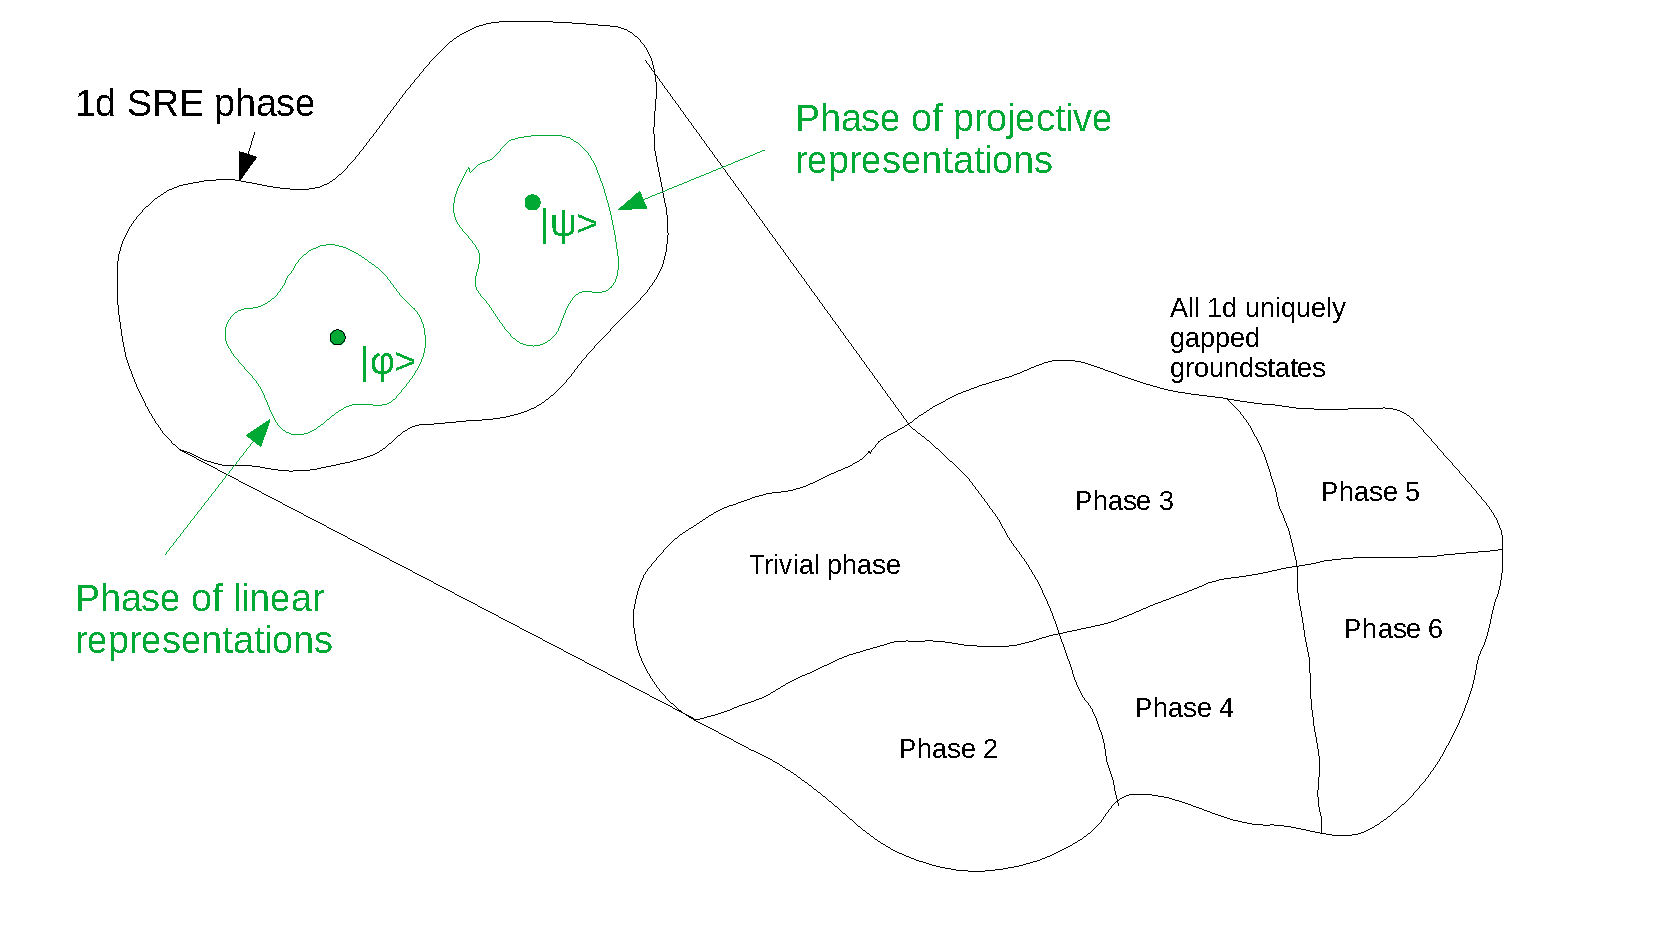
\includegraphics[width=\linewidth]{Figures/SPT_Phases_1d.pdf}
	\end{center}
\end{frame}

\begin{frame}{Edge modes}
	\begin{columns}
		\begin{column}{0.6\textwidth}
			\begin{block}{Definition}
				Edge modes are the ground state degeneracy introduced by introducing an edge.
			\end{block}
			\pause
			E.g. Let $H\in\BB(\HH_L\otimes\HH_R)$ be
			\begin{enumerate}
				\item $G$-invariant.
				\item sum of local therms.
				\item with SPT $\ket{\psi}$ as unique gapped ground-state.
			\end{enumerate}
		\end{column}
		\begin{column}{0.4\textwidth}  %%<--- here
			\begin{center}
				\includegraphics[width=\textwidth]{Figures/Fermi-Hubbard Ladders.pdf}
			\end{center}
		\end{column}
	\end{columns}
\end{frame}

\begin{frame}{Edge modes}
	\begin{columns}
		\begin{column}{0.6\textwidth}
			Eg. Let $H_R\in\BB(\HH_R)$ be the conditional expectation of $H$ to $\HH_R$ then:
			\pause
			\begin{enumerate}
				\item The ground-state of $H_R$ doesn't have to be unique.
				\item The ground state subspace has to be $G$-invariant.
				\item If the SPT index is non-trivial the ground-state of $H_R$ can't be unique (protected ground-state degeneracy).
			\end{enumerate}
		\end{column}
		\begin{column}{0.4\textwidth}  %%<--- here
			\begin{center}
				\includegraphics[width=\textwidth]{Figures/Fermi-Hubbard Ladders.pdf}
			\end{center}
		\end{column}
	\end{columns}
\end{frame}

\begin{frame}{Questions}
	\begin{center}
		
\includegraphics[width=0.5\textwidth]{Figures/AnyQuestions.jpg}
	\end{center}
	\begin{itemize}
		\item I can show some of my own theorems on demand.
	\end{itemize}
\end{frame}

\begin{frame}{Second group cohomology group}
	Let $G$ be a compact lie group.
	\begin{block}{Definition}
		Take $R:G\rightarrow U(\CC^D)$. $R$ is the lift of a projective representation if there exists a $C:G^2\rightarrow U(1)$ satisfying
		\[R(g)R(h)=C(g,h)R(gh).\]
	\end{block}
	\pause
	Because of associativity
	\begin{align*}
		(R(g)R(h))R(l)&=R(g)(R(h)R(l))\\
		C(g,h)C(gh,l)&=C(g,hl)C(h,l).
	\end{align*}
	Such a C is called a 2-cochain ($C\in Z^2$).
\end{frame}

\begin{frame}{Second group cohomology group}
	\begin{block}{Definition}
		We call $C:G^2\rightarrow U(1)$ a coboundary ($C\in B^2$) if there exists a $\beta:G\rightarrow U(1)$ such that
		\[C(g,h)=\beta(g)\beta(h)\overline{\beta(gh)}.\]
	\end{block}
	The second group cohomology group is defined as $H^2(G,U(1)):=Z^2/B^2$.
	\pause
	\begin{block}{Claim}
		The AKLT groundstate cannot be connected to a product state because cochain corresponding to
		\begin{align*}
			R(1,0)&=\sigma^x&R(0,1)&=\sigma^z&R(1,1)&=\sigma^y
		\end{align*}
		is in a nontrivial second group cohomology class.
	\end{block}
\end{frame}

\begin{frame}{1D SPT classification results}
Let $\AA$ be a quasi local algebra over $\ZZ$.
\begin{block}{Theorem 1:}
There exists an $H^2(G,U(1))$ valued index on $G$-invariant SRE states. This index is invariant under $G$-invariant LGA's\footnote{Yoshiko Ogata. A classification of pure states on quantum spin chains satisfying the split property with on-site finite group symmetries. arXiv:1908.08621, 2019.}. (This result is actually more general)
\end{block}
\end{frame}

\begin{frame}{1D SPT classification results}
Let $\AA$ be a quasi local algebra over $\ZZ$.
\begin{block}{Theorem 2:}
If two $G$-invariant SRE states $\omega_1$ and $\omega_2$ have the same $H^2(G,U(1))$-valued index then there exist $G$-invariant product states $\phi_1,\phi_2$ and an LGA $\alpha_1$ such that
\[\omega_1\otimes_{\text{stack}}\phi_1=\omega_2\otimes_{\text{stack}}\phi_2\circ\alpha_1 \footnote{Anton Kapustin, Nikita Sopenko, and Bowen Yang. A classification of invertible phases of bosonic quantum lattice systems in one dimension. Journal of Mathematical Physics, 62(8):081901, Aug 2021.}.\]
\end{block}
\end{frame}

\begin{frame}{Loops of 1D SPT classification results}
Let $\AA$ be a quasi local algebra over $\ZZ$.
\begin{block}{Theorem 3:}
$G$-invariant locally generated loops of invertible states are classified by an $H^2(G,U(1))\oplus H^1(G,U(1))$-valued index. This classification is also complete.\footnote{Sven Bachmann, Wojciech De Roeck, Martin Fraas and Tijl Jappens, A classification of G-charge Thouless pumps in 1D invertible states, https://doi.org/10.48550/arxiv.2204.03763, 2022}
\end{block}
\end{frame}

\begin{frame}{2D SPT classification results}
Let $\AA$ be a quasi local algebra over $\ZZ^2$.
\begin{block}{Theorem 4:}
$G$-invariant SRE's carry an $H^3(G,U(1))$-valued index. This index is invariant under $G$-invariant LGA's.\footnote{Yoshiko Ogata. A $H^3(G,U(1))$-valued index of symmetry protected topological phases with on-site finite group symmetry for two-dimensional quantum spin systems. arXiv:2101.00426, 2021.}
\end{block}
\end{frame}

\begin{frame}{2D translation invariant SPT classification results}
Let $\AA$ be a quasi local algebra over $\ZZ^2$.
\begin{block}{Theorem 5:}
$G$-invariant stably SRE's, that are translation invariant in one direction carry an $H^3(G,U(1))\oplus H^2(G,U(1))$-valued index. This index is invariant under $G$-invariant, translation invariant LGA's.\footnote{Tijl Jappens, SPT indices emerging from translation invariance in two dimensional quantum spin systems, https://doi.org/10.48550/arxiv.2202.11758, 2022}
\end{block}
\end{frame}

\begin{frame}{2D translation invariant SPT classification results}
Let $\AA$ be a quasi local algebra over $\ZZ^2$.
\begin{block}{Theorem 6:}
$G$-invariant stably SRE's, that are translation invariant in two directions carry an
\[H^3(G,U(1))\oplus H^2(G,U(1))\oplus H^2(G,U(1))\oplus H^1(G,U(1))\]
-valued index. This index is invariant under $G$-invariant, translation invariant (in two directions) LGA's.\footnote{Tijl Jappens, SPT indices emerging from translation invariance in two dimensional quantum spin systems, https://doi.org/10.48550/arxiv.2202.11758, 2022}
\end{block}
\end{frame}

\end{document}


